\documentclass[conference]{IEEEtran}

\usepackage[T1]{fontenc}
\usepackage[utf8]{inputenc}
\usepackage{cite}
\usepackage{graphicx}
\usepackage{booktabs}
\usepackage[hidelinks]{hyperref}

\newcommand{\toolname}{\textsc{PerforceLog}}
\newcommand{\beepbeep}{\textsc{BeepBeep}}

\begin{document}

\title{\toolname{}: Detecting Software Process Antipatterns\\
from Perforce Logs with Prometheus Metrics and CEP}

\author{\IEEEauthorblockN{Hanifah}
\IEEEauthorblockA{\textit{D\'epartement d'informatique}\\
\textit{Universit\'e du Qu\'ebec \`a Chicoutimi (UQAC)}\\
Chicoutimi, Canada\\
Email: \textit{to be completed}}
\and
\IEEEauthorblockN{Sylvain Hall\'e, Yannick}
\IEEEauthorblockA{\textit{Supervisors --- UQAC}}}

\maketitle

\begin{abstract}
Game studios journal intense Perforce activity over binary Unreal assets
(\texttt{.uasset}, \texttt{.umap})---process signals come from log
metadata, not textual diffs. \toolname{} parses multi-gigabyte \texttt{p4d}
logs into event blocks, computes offline OpenMetrics metrics (Counter,
Gauge, Histogram, Summary), and applies \beepbeep{} CEP to detect five
VCS-observable bad behaviours mapped to a subset of ReliSA's 168 entries.
On a university UE~5.6 log (16\,262 blocks, ${\sim}$1.7\,GB): 217
edit$\rightarrow$revert alerts, 250 apathy cases, submission peaks of 60
users/hour.
\end{abstract}

\begin{IEEEkeywords}
software process antipatterns, Perforce, Prometheus, CEP, game development
\end{IEEEkeywords}

%======================================================================
\section{Introduction}
\label{sec:intro}
%======================================================================

Collaborative game development relies on Perforce, yet \texttt{p4d} logs are
rarely mined for \emph{process} health. Activity is intense and
heterogeneous---many users, parallel projects, local and remote
connections---over \textbf{binary assets} that cannot be line-merged like
source code; insight must come from command sequences (edit, sync, submit,
revert) and timing.

ReliSA catalogues \textbf{168} software process antipatterns~\cite{relisa_catalogue}.
We define an antipattern operationally as a \textbf{bad behaviour} detectable
from \texttt{user-*} traces; most ReliSA entries (meetings, management,
requirements) leave no \texttt{p4d} footprint. We scope \textbf{five}
VCS-observable behaviours (Table~\ref{tab:relisa}).

\textbf{Contributions.} (1)~A streaming parser assembling \textbf{event
blocks} (command + \texttt{completed} + \texttt{---} metrics by
\texttt{pid}) into a 27-column export; (2)~offline Prometheus-compatible
metrics via \beepbeep{}~\cite{hallé_beepbeep}; (3)~stateful CEP for
temporal patterns beyond aggregates.

%======================================================================
\section{Related Work}
\label{sec:etat}
%======================================================================

\textbf{Process antipatterns.} ReliSA~\cite{relisa_catalogue} formalises
organisational dysfunctions; few works ground detectors in real game-studio
VCS logs. Our scope is deliberately narrow: bad behaviours visible in
Perforce metadata, mapped to the nearest ReliSA fiches as proxies.

\textbf{Observability.} Prometheus defines Counter, Gauge, Histogram, and
Summary~\cite{prometheus_metric_types,prometheus_java_client}; OpenMetrics
standardises exposition~\cite{openmetrics}. Prior VCS studies rarely
reproduce these types offline on full \texttt{p4d} archives.

\textbf{CEP.} Complex event processing~\cite{luckham_cep} maintains state
across ordered events---unlike stateless counters---enabling edit$\rightarrow$revert
and checkout-lifecycle detection. \beepbeep{} integrates CEP pipelines in
Java for batch replay.

%======================================================================
\section{Methodology}
\label{sec:methodo}
%======================================================================

\subsection{Scoped behaviours}
Eleven \texttt{user-*} commands are parsed
(\texttt{edit}, \texttt{submit}, \texttt{sync}, \texttt{revert}, etc.).
Table~\ref{tab:relisa} maps our five detections to ReliSA; some are
\emph{proxies}, not full catalogue coverage.

\begin{table}[!t]
  \caption{Five scoped behaviours vs.\ ReliSA (168 entries).}
  \label{tab:relisa}
  \centering
  \scriptsize
  \begin{tabular}{@{}p{0.22\linewidth}p{0.22\linewidth}@{}}
    \toprule
    \textbf{Detection} & \textbf{ReliSA fiche} \\
    \midrule
    Submission rush & Collective\_Procrastination \\
    Low activity & Warm\_Bodies \\
    High edit/submit & Lone-Wolf \\
    Checkout w/o submit & Bystander\_Apathy (proxy) \\
    Edit$\rightarrow$revert & Cascading\_Branches (approx.) \\
    \bottomrule
  \end{tabular}
\end{table}

\subsection{Pipeline}
Fig.~\ref{fig:arch} summarises \toolname{}. The log is read in streaming
mode; the analytical unit is an \textbf{event block} linked by
\texttt{pid}. Blocks are deduplicated
(\texttt{timestamp|pid|command|args|files}); chronological order is
preserved for CEP. Exports: \texttt{perforce\_events\_v3}, OpenMetrics
JSON, CEP alerts, JFreeChart figures.

\begin{figure}[!t]
  \centering
  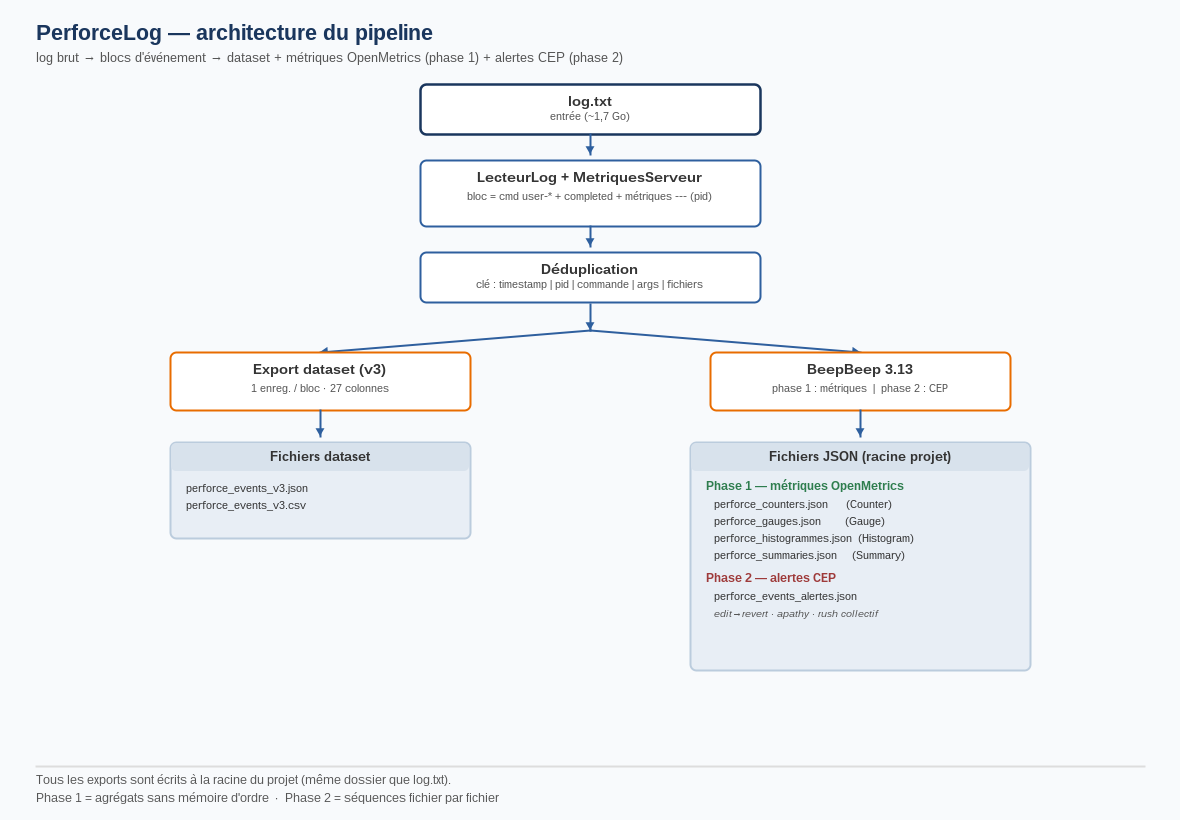
\includegraphics[width=\linewidth]{figures/fig00_architecture_pipeline.png}
  \caption{Pipeline: parse $\rightarrow$ metrics $\rightarrow$ CEP.}
  \label{fig:arch}
\end{figure}

\subsection{Phase~1: Prometheus metrics}
Counters (\texttt{events\_total}, \texttt{submit\_total},
\texttt{edit\_total}); Gauges (\texttt{open\_edit\_files},
\texttt{open\_edit\_users}); Histogram/Summary on
\texttt{command\_duration\_seconds} (buckets 0.05--1200\,s, quantiles
p50--p99). Pipelines:
\texttt{QueueSource}$\rightarrow$\texttt{FilterOn}$\rightarrow$\texttt{Cumulate};
state automaton \texttt{editsOuverts} for open checkouts.

\subsection{Phase~2: CEP}
Stateful detector on \texttt{(user|file)$\rightarrow$last edit}:
\texttt{revert} after \texttt{edit} $\rightarrow$ alert; open files at log
end $\rightarrow$ apathy; $\geq 3$ distinct submitters/hour $\rightarrow$
collective rush. Phase~1 answers ``how much?''; phase~2 answers ``in what
order on this file?''

%======================================================================
\section{Results}
\label{sec:resultats}
%======================================================================

\textbf{Dataset.} ${\sim}$1.7\,GB university log (Unreal Engine 5.6,
NAD/NAND, 26--27 April 2026): 17\,187 raw blocks, \textbf{16\,262}
deduplicated.

\textbf{Phase~1.} 16\,262 events; 1\,224 submits; 4\,069 edits. Gauge
peaks: \textbf{500} open files, \textbf{79} users (27 April, 16:00).
Duration p50\,=\,0.09\,s, p99\,=\,85\,s; \texttt{user-sync} p99\,=\,1\,102\,s.
Warm Bodies proxy: 1\,475 events (top user); Lone Wolf: edit/submit ratio
up to 182. ${\sim}$89\% of commands $<$0.25\,s (histogram); long tail from
heavy binary syncs.

\textbf{Phase~2.} \textbf{217} edit$\rightarrow$revert alerts;
\textbf{250} apathy files (matches final gauge of 250); rush up to
\textbf{60} distinct submitters/hour (27 April, 13:00).

\begin{figure}[!t]
  \centering
  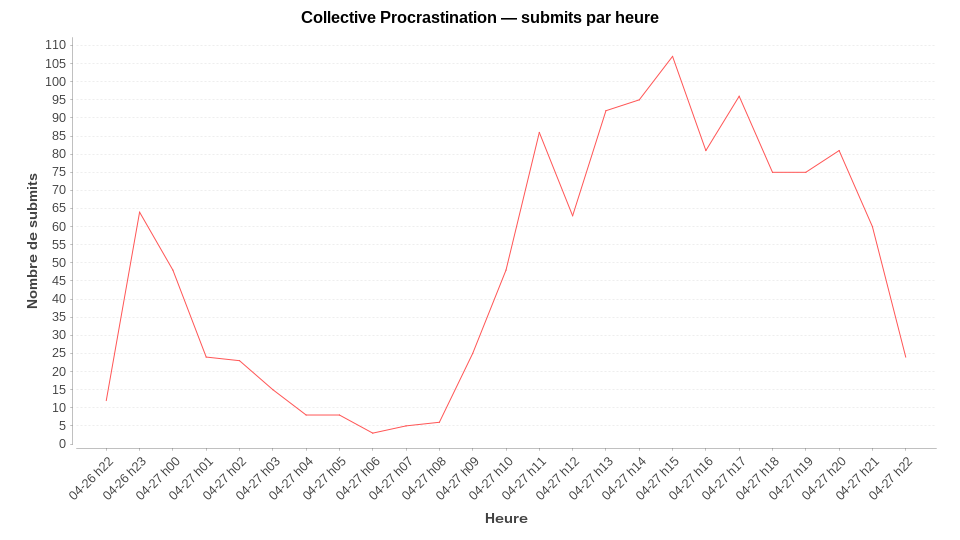
\includegraphics[width=0.48\linewidth]{figures/fig02_submits_par_heure.png}
  \hfill
  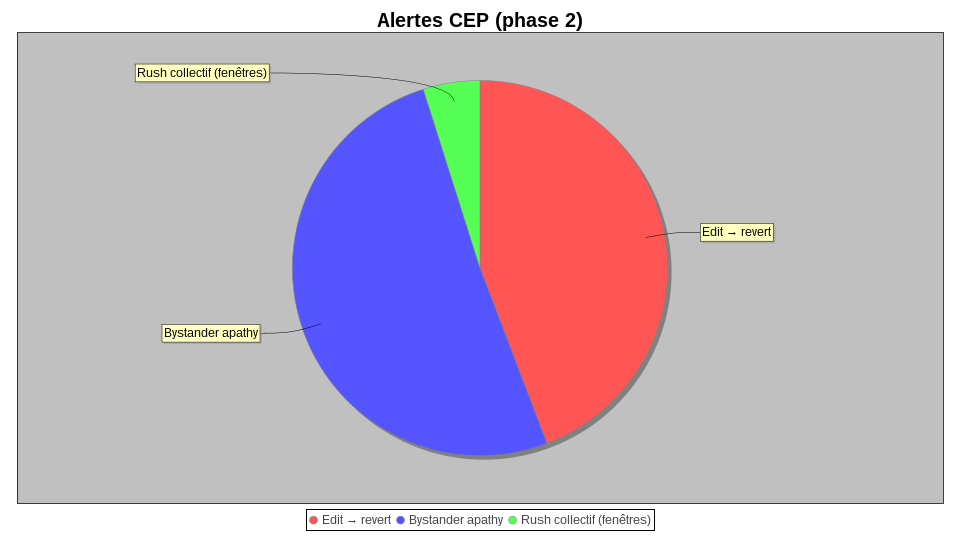
\includegraphics[width=0.48\linewidth]{figures/fig07_alertes_phase2.png}
  \caption{Left: submits/hour. Right: CEP alert counts.}
  \label{fig:results}
\end{figure}

%======================================================================
\section{Conclusion}
\label{sec:conclusion}
%======================================================================

\toolname{} chains raw Perforce logs to OpenMetrics-compatible metrics and
CEP alerts for game-production process analytics. Phase~1 quantifies
activity; phase~2 captures order-dependent behaviours (edit$\rightarrow$revert,
checkout abandonment, submission rushes) invisible to counters alone.
Gauge/apathy agreement (250/250) supports detector consistency.

Submission peaks likely reflect coursework deadlines; high edit/submit
ratios suggest local work with little sharing; long syncs fit catch-up after
infrequent updates on large binary assets, worsened by remote access.

\textbf{Limits.} Five behaviours of 168 ReliSA entries; multi-project log
without official team roster; organisational antipatterns invisible in VCS;
proxies and alerts need qualitative validation (true/false positives).
Single university depot; batch quantiles differ from live Prometheus
windows~\cite{prometheus_metric_types}.

\textbf{Future work.} Alert sampling with instructors; per-file revert
hotspots on binary assets; team roster integration; extended phase~2
detectors. Java sources with \beepbeep{}~3.13 reproduce all exports via
\texttt{Main}.

\bibliographystyle{IEEEtran}
\bibliography{ieee_gem_references}

\end{document}
